\documentclass[tikz,border=8pt]{standalone}
\usepackage[utf8]{inputenc}
\usepackage{amsmath,amssymb}
\usepackage{microtype}
\usetikzlibrary{arrows.meta,calc,positioning}

\definecolor{maroon}{RGB}{122,36,53}
\definecolor{taupe}{RGB}{124,95,88}
\definecolor{gold}{RGB}{154,106,31}
\definecolor{muted}{RGB}{124,116,104}
\definecolor{rule}{RGB}{189,169,132}

\begin{document}
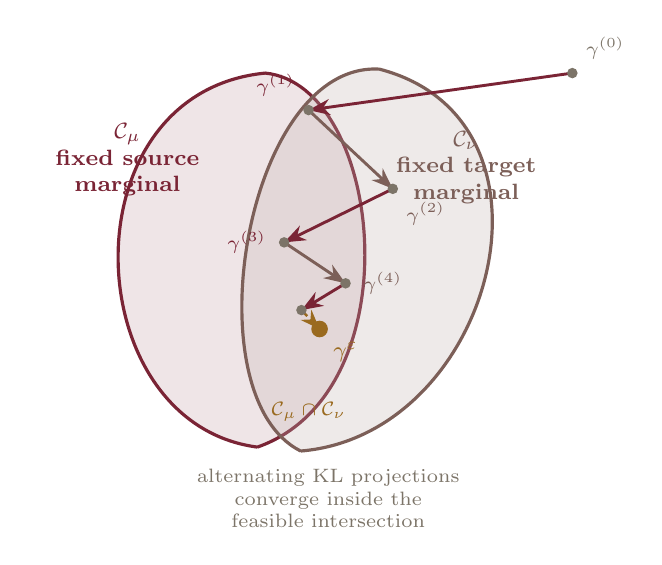
\begin{tikzpicture}[font=\small,>=Stealth,x=1cm,y=1cm]
  \fill[maroon!42,opacity=0.28]
    (3.0,0.4) .. controls (0.7,0.7) and (0.55,4.9) .. (3.1,5.15)
    .. controls (4.6,5.0) and (5.0,1.1) .. (3.0,0.4) -- cycle;
  \draw[maroon,line width=1.15pt]
    (3.0,0.4) .. controls (0.7,0.7) and (0.55,4.9) .. (3.1,5.15)
    .. controls (4.6,5.0) and (5.0,1.1) .. (3.0,0.4);

  \fill[taupe!48,opacity=0.27]
    (3.55,0.35) .. controls (6.0,0.55) and (7.05,4.55) .. (4.55,5.2)
    .. controls (2.85,5.3) and (2.15,1.05) .. (3.55,0.35) -- cycle;
  \draw[taupe,line width=1.15pt]
    (3.55,0.35) .. controls (6.0,0.55) and (7.05,4.55) .. (4.55,5.2)
    .. controls (2.85,5.3) and (2.15,1.05) .. (3.55,0.35);

  \node[maroon,font=\footnotesize\bfseries,align=center,text width=2.3cm]
    at (1.35,4.05) {$\mathcal C_\mu$\\fixed source\\marginal};
  \node[taupe,font=\footnotesize\bfseries,align=center,text width=2.3cm]
    at (5.65,3.95) {$\mathcal C_\nu$\\fixed target\\marginal};
  \node[gold,font=\scriptsize\bfseries] at (3.65,0.85)
    {$\mathcal C_\mu\cap\mathcal C_\nu$};

  \coordinate (g0) at (7.0,5.15);
  \coordinate (g1) at (3.65,4.68);
  \coordinate (g2) at (4.72,3.68);
  \coordinate (g3) at (3.34,3.00);
  \coordinate (g4) at (4.12,2.48);
  \coordinate (g5) at (3.56,2.14);
  \coordinate (gs) at (3.79,1.90);

  \draw[->,maroon,line width=1.05pt] (g0) -- (g1);
  \draw[->,taupe,line width=1.05pt] (g1) -- (g2);
  \draw[->,maroon,line width=1.05pt] (g2) -- (g3);
  \draw[->,taupe,line width=1.05pt] (g3) -- (g4);
  \draw[->,maroon,line width=1.05pt] (g4) -- (g5);
  \draw[->,gold,dashed,line width=0.9pt] (g5) -- (gs);

  \foreach \p in {g0,g1,g2,g3,g4,g5}{\fill[muted] (\p) circle (1.9pt);}
  \fill[gold] (gs) circle (3pt);

  \node[muted,font=\scriptsize,above right=2pt] at (g0) {$\gamma^{(0)}$};
  \node[maroon,font=\scriptsize,above left=2pt] at (g1) {$\gamma^{(1)}$};
  \node[taupe,font=\scriptsize,below right=2pt] at (g2) {$\gamma^{(2)}$};
  \node[maroon,font=\scriptsize,left=3pt] at (g3) {$\gamma^{(3)}$};
  \node[taupe,font=\scriptsize,right=3pt] at (g4) {$\gamma^{(4)}$};
  \node[gold,font=\footnotesize\bfseries,below right=2pt] at (gs)
    {$\gamma^\varepsilon$};

  \node[muted,font=\scriptsize,align=center,text width=4.0cm]
    at (3.9,-0.25) {alternating KL projections\\converge inside the feasible intersection};
\end{tikzpicture}
\end{document}
